\subsubsubsubsection{Entity registry}
\begin{figure}[h]
\centering
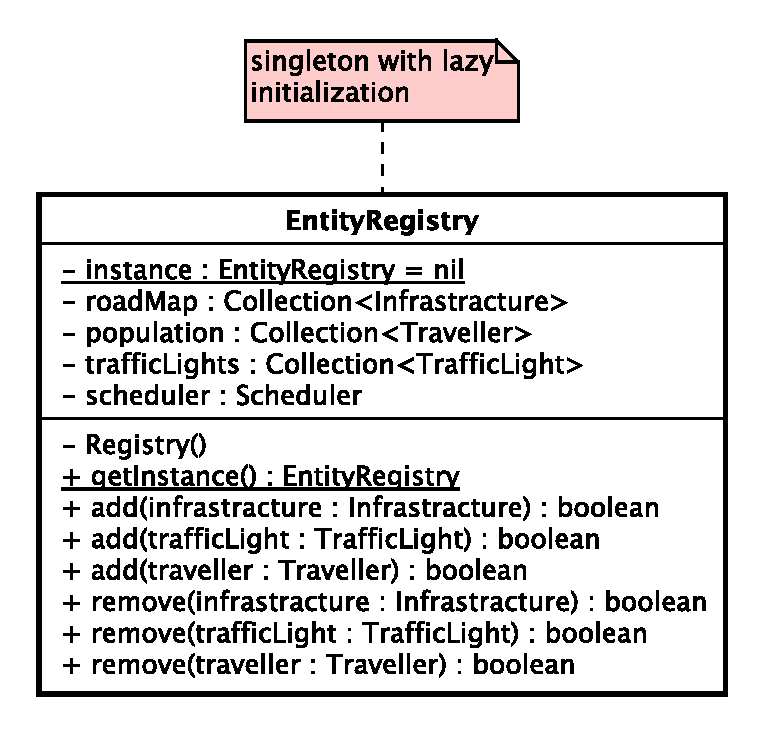
\includegraphics[scale=0.6,keepaspectratio]{images/solution/app/backend/entity_registry.eps}
\caption{\pReactive::EntityRegistry}
\label{fig:sd-app-entity-registry}
\end{figure}
\FloatBarrier
\begin{itemize}
  \item \textbf{\descr} \\
  It represents the urban entity registry of a district.
  Ensures the existence of at most one instance of the class, 
  and provides a global point of access to it.
  Uses lazy initialization, hence no class instance is created 
  or stored until one is first requested.
  It is a singleton because the application layer needs 
  only one master entity.
  \item \textbf{\attrs}
  \begin{itemize}
    \item \texttt{\underline{instance : EntityRegistry = nil}} \\
    A static attribute that contains the unique instance of \texttt{EntityRegistry}.
    It is initialized to nil.
    \item \texttt{roadMap: Collection<Infrastracture>} \\
    The urban entities of the district\footnote{Note that the name 
    \textit{district} is only a convention, indeed it is possible to have a 
    real district splitted into different logical nodes of the system}
    (i.e. crossroads and streets). 
    \item \texttt{population: Collection<MoveableAgent>} \\
    The urban actors that reside on the district.
    \item \texttt{trafficLights: Collection<TrafficLight>} \\
    The traffic lights of the district.
    \item \texttt{scheduler: Scheduler} \\
    The scheduler of agent actions.
  \end{itemize}
  \item \textbf{\ops}
  \begin{itemize}
    \item \texttt{EntityRegistry()} \\
    Private and unique constructor because the class has the exclusive 
    responsability for instancing it.
    \item[+] \texttt{\underline{getInstance() : EntityRegistry}} \\
    Static method lets clients access the unique instance 
    of \texttt{Scheduler}. At the first invocation, it is responsible 
    for creating the instance.
    \item[+] \texttt{add(infrastracture : Infrastracture) : boolean} \\
    Add an infrastracture
    Ensures that the road map contains the specified infrastracture.
    \item[+] \texttt{add(trafficLight : TrafficLight) : boolean} \\
    Ensures that the traffic lights collection contains the specified traffic light.
    \item[+] \texttt{add(agent : MoveableAgent) : boolean} \\
    Ensures that the population contains the specified agent.
    \item[+] \texttt{remove(infrastracture : Infrastracture) : boolean} \\
    Removes a single instance of the specified urban infrastracture from the road map, if it is present.
    \item[+] \texttt{remove(trafficLight : TrafficLight) : boolean} \\
    Removes a single instance of the specified traffic light from the traffic lights collection, if it is present.
    \item[+] \texttt{remove(agent : MoveableAgent) : boolean} \\
    Removes a single instance of the specified agent from the population, if it is present.
  \end{itemize}
\end{itemize} 
